\documentclass{article}

\usepackage{hyperref}       % hyperlinks
\usepackage{url}            % simple URL typesetting
\usepackage{booktabs}       % professional-quality tables
\usepackage{amsfonts}       % blackboard math symbols
\usepackage{nicefrac}       % compact symbols for 1/2, etc.
\usepackage{microtype}      % microtypography

\usepackage{graphicx}
\usepackage{amsmath}
\usepackage{amssymb}
\usepackage{dsfont}

\usepackage{fullpage}
\usepackage{float}
\usepackage[affil-it]{authblk}


\DeclareMathOperator{\Tr}{Tr}
\DeclareMathOperator{\diag}{diag}
\DeclareMathOperator{\cor}{cor}

\newcommand{\beginsupplement}{%
        \setcounter{table}{0}
        \renewcommand{\thetable}{S\arabic{table}}%
        \setcounter{figure}{0}
        \renewcommand{\thefigure}{S\arabic{figure}}%
     }

\title{Phenome-scale causal inference with
bidirectional mediated Mendelian randomization}

\author[1, 2]{Brielin C. Brown \thanks{bb2991@columbia.edu}}
\author[2, 3, 4]{David A. Knowles \thanks{dak2173@columbia.edu}}

\affil[1]{Data Science Institute, Columbia University, New York, NY}
\affil[2]{New York Genome Center, New York, NY}
\affil[3]{Department of Computer Science, Columbia University, New York, NY}
\affil[4]{Department of Systems Biology, Columbia University, New York, NY}

\begin{document}
\maketitle

\begin{abstract}
%Inference of directed biological networks from large-scale observational
%genomics datasets is a long-standing challenge, with relevance to detecting
%core genes under the omnigenic model of complex traits, and understanding risk
%factors for disease more broadly. A well-known problem with observational data
%is the possibility of unobserved confounding. Recently, Mendelian randomization
%(MR) has received attention as a class of methods for inferring causal effects
%in observational data by using genetic variants (SNPs) from genome-wide
%association studies (GWAS) as instrumental variables. However, the application
%of MR to networks of phenotypes presents several unique challenges. First, MR
%infers the total causal effect (TCE) of an exposure on an outcome, which may be
%mediated by other mechanisms in the dataset. Second, MR is usually applied to
%estimate the effect of a fixed exposure on a fixed outcome, but network
%inference requires we also infer the effect of the outcome on the exposure.
%This is sometimes referred to as bi-directional MR (BDMR). Our solution consists of two
%parts. First, we introduce a simple new method for Egger weighting which
%relies on the observation that valid MR instruments must explain less variance
%in the outcome than the exposure. Second, we show that inferring the causal
%direct effects from the matrix of TCE can be thought of as a sparse matrix
%inverse problem, analogous to the graphical lasso. We introduce a new method
%for this problem that allows for the inference of directed edges given an
%arbitrary weighting of the input matrix, allowing us to incorporate TCE
%estimates with large standard error or that are missing entirely.
\end{abstract}

\section{Introduction}
Recent developments in the understanding of complex-trait genetics have
lead to a call for increased study of biological networks (CITE omnigenics 1-2, visscher).
However, interrogating the structure of networks is notoriously difficult,
owing to factors such as unmeasured confounding and reverse causation (CITE?).
In spite of these challenges, modern population-scale biobanks 
offer unprecedented opportunity to study biological networks
 because they can contain simultaneous measurements of
traits, molecular markers and genetic variation  (CITE ukbb, bbjp).

Mendelian randomization (MR) has recently received increased attention as a class of methods
that can mitigate issues in causal inference
 by using genetic variants (SNPs) from genome-wide
association studies (GWAS) as instrumental variables to determine the effect
of an exposure (A) on an outcome (B). To find causal effects,
MR methods must make strong assumptions that limit their
ability to be applied at the phenome-scale. Perhaps the most
controversial assumption is that the SNP only effects B through A
(\textit{i.e.} there is no horizontal pleiotropy). Recent methods such as Egger
regression and the mode-based-estimator are able to relax this assumption, instead
assuming there is no correlated pleiotropy or modal pleiotopy, respectively (CITE egger, mbe).
Another approach, the latent causal variable (LCV) model, is able to detect genetic causality
under arbitrarily-structured pleiotropy (CITE LCV). However, the quantity that LCV
calculates is not interpretable as the effect size of A on B. Most MR studies
also presuppose the direction of effect, specifying one phenotype as the outcome and
the other as the exposure. This is sound when the outcome
is clearly biologically downstream of the exposure, but in many cases it is better
to learn the direction of the effect from the data. Some researchers have instead
used bi-directional Mendelian randomization (gwas-pw) (CITE bimr, pickrell).
However, the utility of this approach for complex traits,
which might contain non-causal genetic correlation,
is questionable (CITE LCV).

In mimicking a randomized controlled trial, MR estimates the
total causal effect (TCE) of A on B (CITE ??). This effect may be mediated by
any number of factors. The proliferation of phenome-scale datasets
allows researchers to simultaneously measure the effects of many possible mediators,
enabling the conversion of TCE estimates into causal direct effect (CDE)
estimates, which are not mediated by any other measured factor.
This raises another disadvantage of approaches such as LCV and gwas-pw. Assuming that either
A causes B or B causes A, but not both, is equivalent to assuming
that the underlying causal network
lacks cycles, which are thought to be an important part of real biological networks (CITE ??).

Here, we introduce an approach called
\emph{bi-directional mediated Mendelian randomization} (bimmer)
for inferring sparse networks of causal direct effects from phenome-scale
GWAS summary statistics.
Our approach has two parts. First, we perform bi-directional Mendelian randomization
between every pair of phenotypes using Egger regression with a
modified SNP selection and weighting scheme that dramatically reduces the
influence of pleiotropic SNPs.
This gives an estimate of the TCE of each phenotype on every other (Figure~\ref{figure0}a-b).
Second,
we perform a causal mediation analysis to convert the matrix
of total causal effects into a sparse, directed network of causal direct effects.
We show that this can be modeled as an $L_1$-regularized matrix inverse problem,
drawing analogy to the graphical lasso (CITE glasso), and introduce a new
method for finding a sparse inverse to a partially-observed matrix called
\emph{inverse sparse regression} (inspre, Figure~\ref{figure0}b-c).
We show in extensive simulations that our approach is able to learn causal
 network structures even in the presence of non-causal genetic correlation.
We apply our method to NNN phenotypes from the UK Biobank, finding thousands
 of direct and indirect causal effects.
 
 
\begin{figure}\label{figure0}
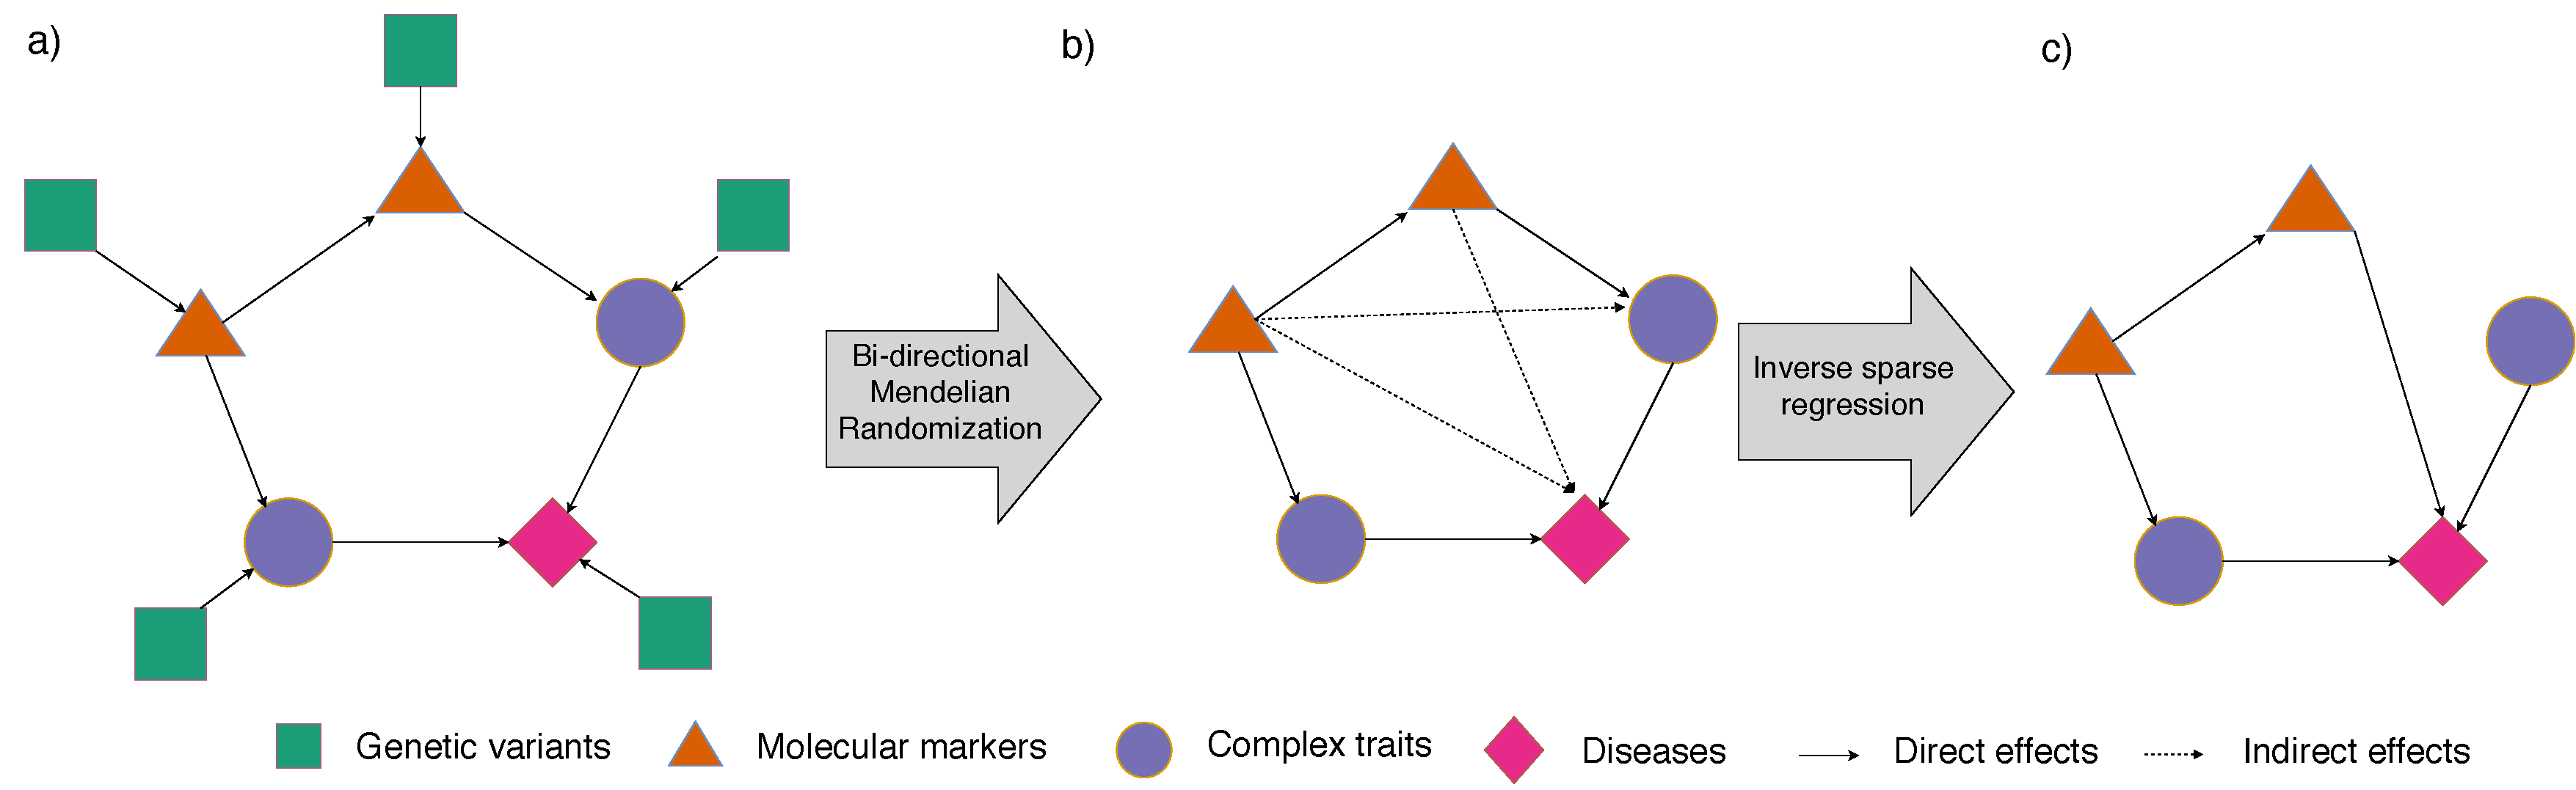
\includegraphics[width=\textwidth]{figures/bimmer_figure1.pdf}
\caption{a) Modern biobanks contains measurements of genetic variants (green squares), molecular markers
(orange triangles), complex traits (purple circles) and diseases (pink diamonds). Genetic variants
effect these phenotypes which in turn effect each other. b) Bi-directional Mendelian randomization
estimates the total causal effect of the phenotypes on each other, which includes both
direct (solid arrow) and indirect (dashed arrow) effects. c) The direct effects can be
found by estimating a sparse approximate inverse to the matrix of total effects, a process we
call inverse sparse regression.}
\end{figure}

\section{Results}
\subsection{Overview of model}
We model each phenotype as a function of 1) time-invariant genetic factors, 2)
time-invariant environmental factors, and 3) other phenotypes at the previous
time-point.
Assume we have $N$ individuals, $D$ phenotypes and $M$ SNPs,
with $Y_t$ be the matrix of phenotypes indexed by time $t$, $X$ the genotype
matrix, $\beta$ the SNP effect matix and $\gamma$ a matrix of unknown
environmental effects. We denote by $R$ the $D \times D$ matrix of
causal direct effects, with $R_{i, j}$ the CDE of phenotype $i$ on
phenotype $j$. We assume that phenotypes do not effect themselves ($R_{i,i} = 0$),
and that the network is sparse ($R$ has many entries that are $0$).
Our goal is to estimate $R$ given summary statistics
 for the association of the genotypes $X$ with the phenotypes measured when
 the system has reached equilibrium, $Y = Y_{t}$.
 Our trait model is
\begin{equation}
Y_{t+1} = Y_{t} R + X\beta + \gamma
\end{equation}
which converges to $Y = (X\beta + \gamma)(I-R)^{-1}$ at equilibrium if the largest eigenvalue
of $R$ has magnitude below 1.

Let $R^{TCE}$ be the matrix of TCE estimates from MR, with $R^{TCE}_{i,j}$ the total
causal effect of phenotype $i$ on phenotype $j$ and $S_{i,j}$ it's standard error.
We show~\ref{methods} that
in this model,
\begin{equation}\label{r_cde_main}
R = I - R^{TCE^{-1}} D[1 / R^{TCE^{-1}}]
\end{equation}
where $D$ is an operator that sets all off-diagonal elements to 0, and $/$
represents element-wise division.

In practice, the matrix $R^{TCE}$ need not be well-conditioned or
 even invertible, leading
to challenges when solving~\ref{r_cde_main}. Instead of calculating an exact
or psuedo-inverse, we exploit the assumption that the underlying graph of
CDE is sparse. Specifically, we seek matrices $U$ and $V$ such that $VU=I$, $U \approx R^{TCE}$
and $V$ is sparse. We find them by solving the following constrained optimization problem,
\begin{equation} \label{opt_main}
\min_{\{U, V : VU = I\}} \frac{1}{2} ||W \circ (R^{TCE} - U)||_F^2 +
   \lambda \sum_{i\neq j}|V_{ij}|
\end{equation}
where $W = W_{i,j} = 1/S_{i,j}^2$ is a set of per-entry inverse variance weights,
and $\lambda$ is the LASSO shrinkage parameter (CITE LASSO, glasso). Note that in
this method, missing entries in $R^{TCE}$ can be accommodated simply
by setting their weights to 0.

Some intuition for ~\ref{r_cde_main} can be gained by considering the problem
of estimating a matrix of partial correlations for a set of observed variables.
Analogous to the CDE, the partial correlation measures the degree to which two
variables are correlated while controlling for the effect of all other measured
variables. Given a matrix of observed (standard) correlations, $\Sigma$, the matrix of
partial correlations is $P = D[\Sigma^{-1}] \Sigma^{-1} D[\Sigma^{-1}]$. One of
the most common approaches to calculating $\Sigma^{-1}$, also called
the precision matrix, is the graphical lasso (glasso). This method works
by assuming the data come from a multivariate normal distribution with a sparse
precision matrix, and maximizing the data likelihood with a LASSO penalty.

 We choose the
regularization parameter $\lambda$ by randomly setting entries of the weight matrix to 0 and
evaluating the stability of the resulting graph. This is analogous to the
stability approach to regularization selection(CITE stars), except we exploit the
ability of our method to handle missingness in $R^{TCE}$ to induce variance in the graph rather
than splitting the input matrices, which would require individual-level data.
In each of $10$ cross-validation iterations, we randomly set $20\%$ of $W$ to $0$
and then use inspre to infer the matrix $R$ for various values of $\lambda$.
We use these results to estimate the probability
that each edge is included in the graph under random masking, and use these probabilities
to infer a stability score $\hat{D}$ - roughly corresponding to the fraction of times
that two graphs with the same $\lambda$ disagree on the inclusion of an edge,
 averaged over all edges.
We set $lambda$ to the largest value which gives a stability score $\hat{D} < 0.05$.
For complete details see Section~\ref{methods}.


This leaves the problem of producing a good estimate for $R^{TCE}$,
which can be challenging when there is non-causal genetic correlation or
differential power across phenotypes. Most MR studies use the set of
genome-wide significant (GWS, $p \le 5\times 10^{-8}$) SNPs for a trait as instruments.
Instead, we exploit the observation that if $A$ causes $B$ and a SNP effects $A$ directly,
the effect of the SNP on $B$ can be no larger than the effect of the SNP on $A$ times
the effect of $A$ on $B$. That is, the SNP must have it's per-variance contribution to
$B$ reduced by the network. We use this intuition to construct a new
weighting scheme for Egger regression.
First, we select a $p$-value threshold $p$. For every phenotype $i$, we
 construct a set of marginally associated SNPs at threshold $p$. Next,
 for every ordered pair of phenotypes $i, j$, we consider only SNPs that reach
 signficance level $p$ in phenotype $i$ but not $j$. For this set of SNPs, we calculate
 a weight based on the Welch test statistic for a two-sample difference in mean
 and the standard inverse-variance weight. If $\hat{\beta}_{k, i}$ is our estimate
 of the effect of SNP $k$ on phenotype $i$ and $\hat{s}_{k, i}$ it's standard error,
 our weight is,
\begin{equation}
w^{i,j}_k = \frac{|\hat{\beta}_{k, i}| - |\hat{\beta}_{k, j}|}
  {\sqrt{\hat{s}_{k,j}^2 (\hat{s}^2_{k, i} + \hat{s}^2_{k, j})}}
\end{equation}
We use these SNP weights in the Egger regression of $j$ on $i$.
To avoid bias, this means that we must use two sets of summary
statistics: one set for SNP selection and weight construction,
 and the second set for $R^{TCE}$ estimation.


\subsection{Simulations}
\subsubsection*{Bi-directional Mendelian randomization}
Our first goal was to assess whether our weighted Egger regression approach
had a well-controlled type-I error rate (FPR) under the two-way null. To this
end we simulated GWAS summary statistics for two phenotypes with $M=1,000,000$
independent SNPs, $20\%$ heritability and $N = 100,000$ individuals in both
 the SNP discovery and effect estimation cohorts. In each simulation, there
 were $5,000$ causal
SNPs per phenotype. In our first simulation, $1,000$ of these SNPs are pleiotropic,
effecting both phenotypes, but with no correlation of their effects. In our
second, these $1,000$ SNPs are again shared, but with correlated pleiotropy
for a total genetic correlation of $\rho_g = 0.2$. In our final simulation under the
null, we again have $\rho_g = 0.2$, except the studies have very different sample sizes
($N_1 = 200,000$, $N_2 = 50,000$) and shared effects are twice as large on average
in the smaller cohort. This makes shared SNPs much more likely to have
low $p$-values in the second cohort. In each setting, we compared our approach
against the standard approach of Egger regression using all SNPs reaching GWS for
 the exposure as instruments, as well as an oracle with access to the true
effect sizes that uses only non-pleiotropic SNPs.

In the first setting, uncorrelated pleiotropy, all methods were able to 
effectively control the FPR at level $\alpha = 0.05$ in both directions
(Figure~\ref{figure1}a, Table~\ref{table1}).
In the second setting, correlated pleiotropy,
standard Egger regression produced excess false-positives, but our weighting
scheme is able to reduce the false positive rate substantially
(Figure~\ref{figure1}b, Table~\ref{table1}).  In the most challenging setting,
correlated pleiotropy with unequal power, standard Egger regression produces
many excess false positives in both directions, but our weighting scheme
again substantially reduces the error rate, from $0.284$ to $0.087$ in
the $A\rightarrow B$ direction and from $0.492$ to $0.029$ in the 
$B\rightarrow A$ direction (Figure~\ref{figure1}c, Table~\ref{table1}).

\begin{figure}\label{figure1}
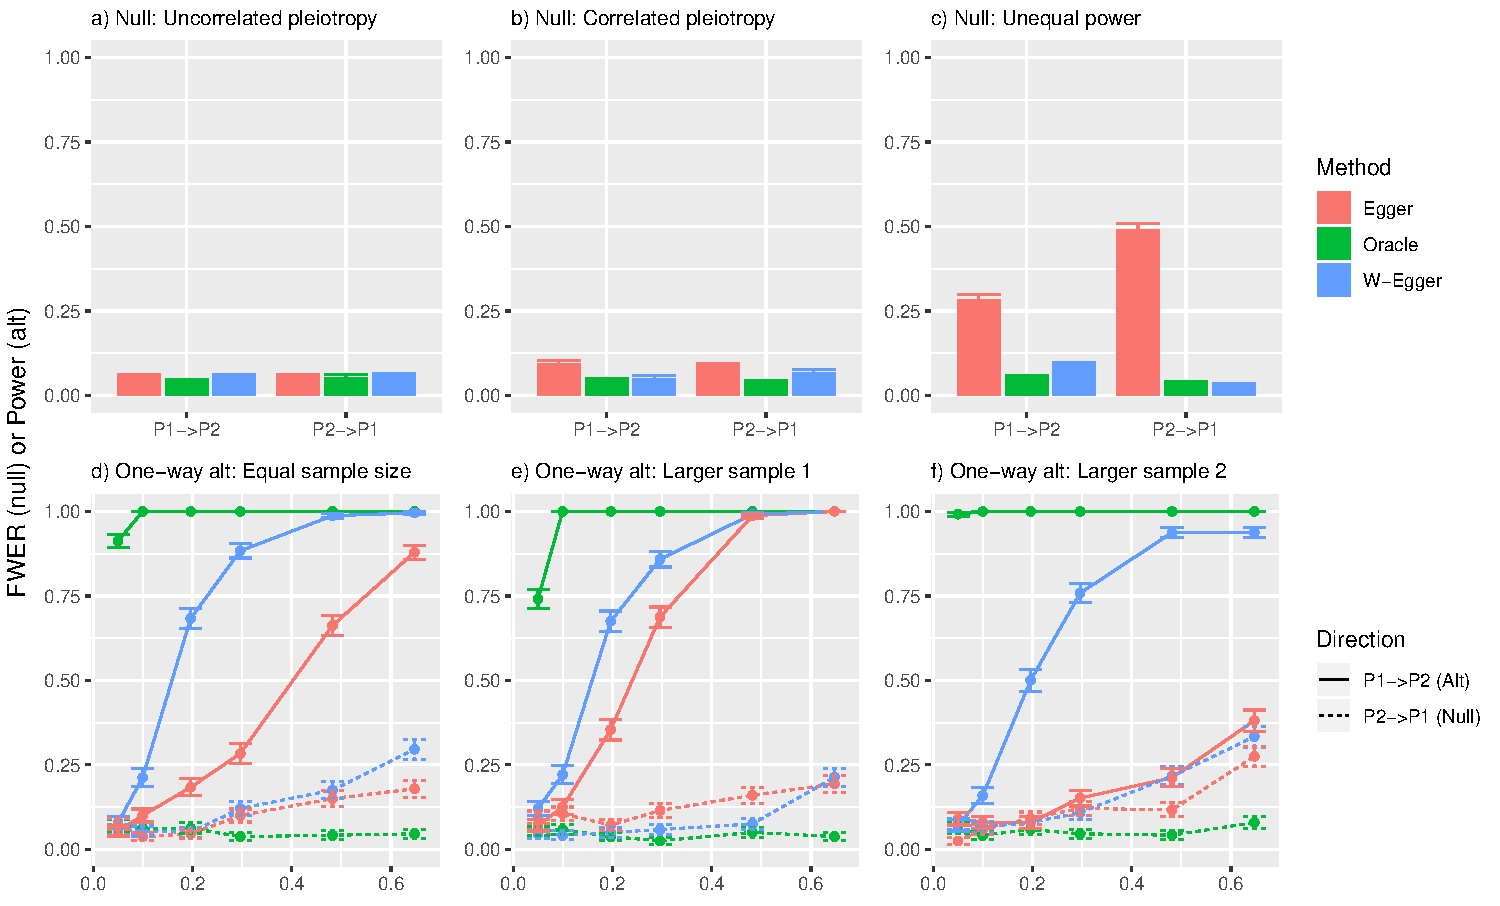
\includegraphics[width=\textwidth]{figures/figure1.pdf}
\caption{We simulated GWAS summary statistics for two phenotypes ($A$, $B$) with $M=1,000,000$
independent SNPs, $20\%$ heritability and $N = 100,000$ individuals in both
 the SNP discovery and effect estimation cohorts. In each simulation, there
 were $5,000$ causal SNPs per phenotype. a) Both the effect of A on B and B on A are null,
 and $1000$ of the SNPs have uncorrelated pleiotropic effects. All methods are well behaved.
 b) Both effects are again null, but the $1000$ shared SNPs have equal effects on both
 phenotypes. Egger regression results in excess false positives which our weighting scheme
 reduces. c) Both effects are null and the shared SNPs have an equal effect on both phenotypes,
 but the shared SNPs have twice as large an effect on $B$, which also has a much smaller sample
 size. Egger regression results in numerous false positives, which our weighting scheme corrects.
 d) $A$ has a variable effect on $B$ and the studies have equal sample size. Our weighting
 scheme improves power over standard Egger regression. e) $A$ effects $B$, which has a much
 lower sample size. Our weighting scheme improves power, but not as much as in (d). f) $A$
  effects $B$, but $A$ has a much smaller sample size. Our weighting scheme substantially increases
  power. We conduced $1000$ simulations for each null experiment (a-c) and $250$ simulations
  per effect size for each alt experiment (d-f). }
\end{figure}

Next, we wanted to asses the power of our approach under the one-way alternate
hypothesis for various effect sizes. We again conduct thee simulations,
calculating the power for effect sizes ranging from $0.05$ to $0.7$.
In the first, the cohorts had equal sample sizes. In the second, the exposure
cohort has larger sample size, and in the third the outcome cohort
has a larger sample size. In all settings, our weighted Egger approach shows
a substantial gain in power over standard Egger regression. This is especially
notable for smaller effect sizes, and when the outcome GWAS is larger.
In this latter setting, the power of standard egger regression is only slightly
higher than the FPR for the null hypothesis on the reverse direction,
while our weighted Egger regression has very high power
(Figure~\ref{figure1}d-f, Table~\ref{table2}). However, both
methods suffer from an increase in false positives in the reverse direction
when the effect size in the forward direction is strong. For more on this
phenomenon, see~\ref{discussion}.


Finally, we tested the power of our approach under the two way alternate
hypothesis. We tested pairs of effects ranging from $-0.5$ to $0.5$ in both cohorts.
Here we conduct two simulations: one with equal sample size of $N=100,000$,
and one unequal sample sizes $N_1 = 200,000$ and $N_2 = 50,000$.
In all settings, our approach improves power
substantially over standard Egger regression (Figure~\ref{figure2}a-d). As with
the one-way alt, this is particularly apparent when the outcome has a larger
sample size than the exposure (Figure~\ref{figure2}d). We also observed that both
methods had lower power when $R_{12} \approx -R_{21}$ and vice versa, especially when
both are large. Indeed, as $R_{12} \rightarrow -R_{21} \rightarrow 1$, the model
becomes unidentifiable. This setting is actually a violation of the \emph{faithfulness}
assumption commonly employed in causal inference (CITE ??).

\begin{figure}\label{figure2}
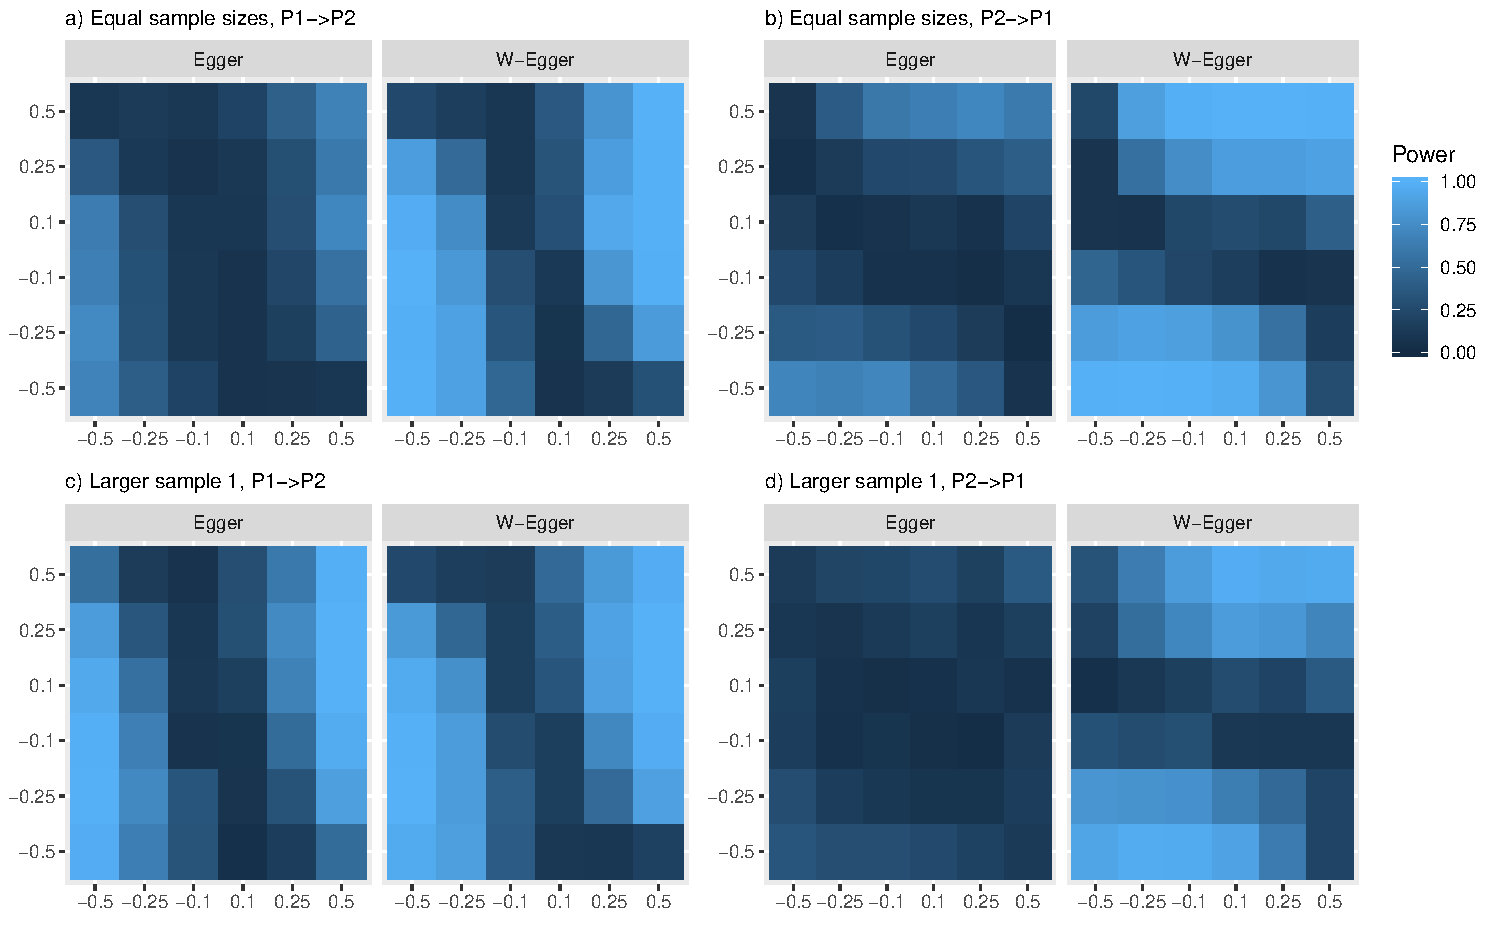
\includegraphics[width=\textwidth]{figures/figure2.pdf}
\caption{We simulated GWAS summary statistics for two phenotypes ($A$, $B$) with $M=1,000,000$
independent SNPs, $20\%$ heritability and $N = 100,000$ individuals in both
 the SNP discovery and effect estimation cohorts. In each simulation, there
 were $5,000$ causal SNPs per phenotype of which $1,000$ were shared with uncorrelated
 effect sizes. a) Power to detect the effect of $A$ on $B$ when the studies have equal
 sample sizes. Our weighting scheme increases power of standard Egger regression, but both
 methods struggle to detect when the traits cancel each other out. b) Power to detect the
 effect of $B$ on $A$. Our approach improves power and the cancellation pattern is transposed.
 c) Power to detect the effect of $A$ on $B$ when $A$ has a larger sample size. Our approach
 improves power, though both do well. d) Power to detect the effect of $B$ on $A$ when
  $A$ has a larger sample size. Our approach improves power substantially over standard
  Egger regression, which struggles to detect the effect.}
\end{figure}

In these simulations, we used a $p$-value threshold of $5\times 10^{-6}$
for all wighted Egger regresssion analyses. We tested $p$-value thresholds
ranging from $5\times 10^{-4}$ to $5\times 10^{-8}$, and found similar
results compared to standard Egger for all thresholds. We found that
$5\times 10^{-6}$ provided a nice balance between increased power under 
the alt and control of the type-I error rate under the null. However, lower
cutoffs will provide better control of the type-I error rate in difficult situations
at the expense of reduced power. Like-wise, higher cut-offs yield higher power
while reducing control of the type-I error rate
(Tables~\ref{supptable1} and ~\ref{supptable2}). 

\subsubsection*{Inverse sparse regression}
As detailed above, both inspre and glasso can be viewed as methods
for finding a sparse, approximate inverse to a noisily measured matrix.
Therefore, we sought to compare these two methods when data are simulated
from the glasso model. We generated data
from a multivariate-normal distribution with a sparse precision matrix
for various graph structures, sample sizes, and numbers of features.
We considered three kinds of graph structures: 1) Erdos-Reyni random graphs,
where each edge is included with probability $p$, 2) hub graphs, where nodes
are partitioned into
disjoint sets and every node in each set is connected to a central "hub" vertex,
3) scale-free networks, where the vertex degree distribution
follows a power law. Hub and scale-free networks are intended to mimic common
biological networks (CITE ??). In each setting we calculated the precision,
the number of true edges among all inferred edges, and recall, the proportion
of true edges detected. We used these to calculate the $F_1$ score, the
harmonic mean of precision and recall (CITE ??), as a function of the
stability of the inferred graph. For the graphical lasso, we used StARS to
evaluate graph stability. For inspre, we used random masks in the weight matrix
as detailed above. As suggested in (CITE stars), we focus on the crucial
region of stability around $\hat{D} = 0.05$.

First, we simulated data with $40$ features and $800$ samples. Our random
graphs included each edge with probability $p=0.04$, and our hub graphs had
two hubs of $20$ features each. In this setting inspre and glasso performed
similarly for all graph types, with glasso performing slightly better on
random graphs, inspre performing slightly better on hub graphs, and 
both methods having very similar performance for scale-free graphs
(Supplmental Figure~\ref{figureS1}a-c). Next, we simulated  data with $100$
features and $500$ samples. Here our random graphs included each edge with probability $p=0.02$ and our hub graphs had $5$ hubs. In this setting, glasso outperformed inspre on
random graphs, inspre outperformed glasso on hub graphs, and both methods again
had similar performance on scale-free graphs, with a slight edge towards
glasso (Figure~\ref{figureS1}d-f).

We hypothesized that if the entries in the correlation matrix had variable
sample sizes, the ability of inspre to incorporate weights would improve
performance. This represents a common real-world setting in
which some features are measured on many samples, and some are measured
on only a few. In each simulation, we first chose a maximum missingness
threshold $m$ uniformly between $50\%$ and $99\%$. Then we simulated data with
$100$ features and $2000$ samples. For each feature, we uniformly chose
a random number between $0$ and $m$ and set that proportion of the features
samples to NA. We then calculated the sample correlation matrix using only
samples where both features were measured per pair of features.
In this setting, inspre was able to continue producing accurate
results even with when the maximum misssingness was high. On the other
hand, glasso was not able to produce results at all when there was high
missingness, instead returning a matrix of NA values
(Figure~\ref{figureS2}).



\subsubsection*{Bi-directional mediated Mendelian randomization}
Our final goal was to show that bi-directional Mendelian randomization
could be combined with inspre to fit networks of simulated phenotypes
from phenome-scale GWAS summary statistics. At the time of this writing
we are not aware of any other methods for this specific problem. However,
there are a few approaches to related problems that could be applied.
Specifically, the CDEs between multiple exposures and a single outcome
can be calculated from a multiple regression of SNP effects on the outcome
against SNP effects on the exposures (CITE mvmr). This approach can be used
to find sparse effects by using a LASSO or elastic net regression (elnet-Egger). A more
sophisticated approach, such as MR-Beyesian model averaging (MR-BMA), could also be
applied (CITE MR-bma).

First, we simulated summary
statistics for $50$ phenotypes with $1000$ shared and $2000$ private
causal effect SNPs per pair of phenotypes, $125,000$ total SNPs. Each
phenotype had $20\%$ heritability. The causal
network underlying the phenotypes came from an Erdos-Reyni random graph with
randomly oriented edges. We found that MR-BMA outperformed comparably to
elnet-Egger, but that they both performed poorly compared to inspre.
Moreover, MR-BMA took about $20$ times longer than inspre to run with
default parameter settings (Figure~\ref{figureS4}).

Next, we performed larger-scale simulations with $100$ phenotypes and
$250,000$ total SNPs. We again
simulated data from Erdos-Reyni, hub, and scale-free networks. In this setting
both the graph structure and the orientation of the graphs edges are important
variables to consider. The edge orientation will not necessarily be random:
for example, master regulators would have very high out-degree but low in-degree (CITE ??).
For all graph types, we tested three ways of orienting the edges in the graph:
 1) randomly set the orientation
of each edge (random), 2) preferentially orient edges towards high-degree nodes (towards),
 and 3) preferentially orient edges away from high-degree nodes (away). See
 Figure~\ref{figure4}a-c for examples of different kinds of graphs with
 different edge orientations. We excluded
MR-BMA from these simulations due to runtime concerns.

We found that bimmer was able to accurately re-construct all graph types and edge
orientations considered, while
elnet-Egger consistently had poor performance (Figure~\ref{figure4}d-i, Figure~\ref{figureS3}).
 For random graphs, we found that edge orientation did not have an effect on the
 performance of bimmer. This is possibly because the node degree distribution
 doesn't have enough variance to have nodes that consistently pull edges towards
 or away from them in the latter scenarios. For scale-free and hub graphs, we
 found that bimmer performed better when high-degree nodes had edges oriented
 away from them (Figure~\ref{figureS3}). This is particularly interesting as
 it corresponds to the most likely real-world scenario (CITE ??).

\begin{figure}\label{figure4}
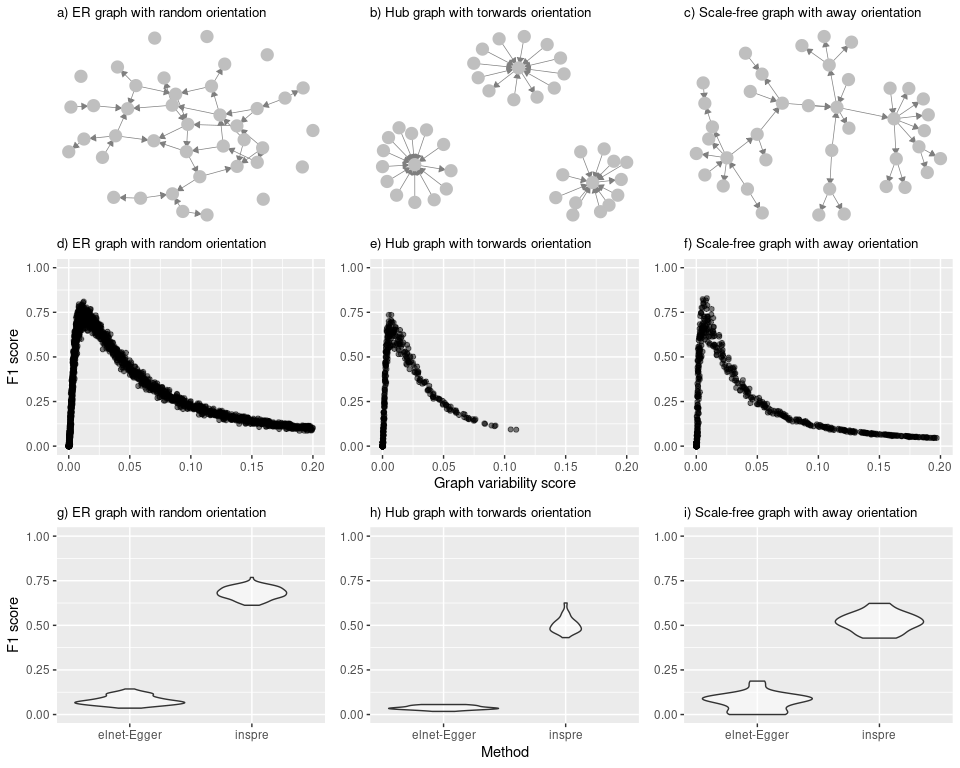
\includegraphics[width=\textwidth]{figures/figure4.png}
\caption{We simulated summary statistics for $100$ phenotypes with $3000$ causal
effects each, $1000$ of which were shared with uncorrelated effects per pair of phenotypes.
We varied the structure and edge orientation of the causal graph underlying the phenotypes.
a) An Erdos-Reyni random graph with randomly oriented edges. Each edge is
included with probability $p=0.05$ and then randomly assigned an orientation. b) A hub
graph with edges preferentially oriented towards high degree nodes. The nodes are split into
three sets and each node in each set is assigned to a central hub vertex. c) A scale-free
graph with edges preferentially oriented away from high degree nodes. These graphs have
node degrees that follow a power-law distribution. We show the $F_1$-score of the method
against the calculated variability score for d) random, e) hub and f) scale-free graphs.
In all cases, we are able to produce accurate results when the variability score is between
about $0.01$ and $0.05$. We also compared the performance against Egger regression
with elastic-net shrinkage at a graph variability score of $0.025$. elnet-Egger
performs quite poorly compared to bimmer.
}
\end{figure}


\subsection{Application to NNN traits from the UK Biobank}



\section{Discussion}\label{discussion}
As biobanks continue to grow in size and scope, new methods that are able to
leverage their power while overcoming common pitfalls will be required.
These datasets offer unprecedented opportunity to study
the causal relationship between molecular markers, complex traits and diseases.
We have introduced bi-directional mediated Mendelian randomization (bimmer),
a novel approach to inferring sparse causal networks from phenome-scale
GWAS summary statistics. We have shown through extensive simulations that
bimmer is able to learn causal graph structures even in the presence of non-causal genetic
correlation and differential power across phenotypes. We applied bimmer to 
NNN phenotypes from the UKBB and found...


While we are not aware of other methods for this problem, our approach
builds on recent MR literature. In particular, multi-variable Mendelian
randomization methods are able to compute causal direct effects when there
are multiple potential exposures and a single outcome (CITE mvmr, MR-BMA). While
these methods work well in that setting, we have shown that they are not well-suited
to the more general problem that we consider here. Another approach, network
Mendelian randomization, calculates the effect of an exposure on an outcome while
accounting for the effects of a third variable (CITE netmr). Our method can
be thought of as a generalization of this approach to an arbitrary number of phenotypes
without pre-specifying any as exposures or outcomes. The first step in our method
involves bi-directional MR with Egger regression weights that reduce the effect
of pleiotropic SNPs. This is related to several recent methods.
In particular, gwas-pc uses asymmetry in the effect size distributions
to choose an effect direction between the two phenotypes. Similarly, 
LCV uses this asymmetry to fit a latent variable model, where imbalanced
genetic correlation between the phenotypes and latent variable imply
the effect direction. Compared to these methods, our approach offers several
advantages. First, like LCV but unlike gwas-pc, our method controls the type-I error rate
when there is non-causal genetic correlation and differential power. Second, like gwas-pc,
but unlike LCV, our method estimates a quantity that is interpretable as the
effect of one phenotype on the other. Finally unlike both,
we are able to estimate both effect directions simultaneously, allowing our
model to accomodate graphs with cycles.

However, our approach also has several disadvantages. First, our method
requires that we split the initial cohort into instrument discovery and
effect estimation sub-cohorts. This is common in MR methods, but LCV has
the distinct advantage of using all SNPs, which obviates the need
for sample splitting and might improve power. Second, while there are some
phenotype pairs where a direct cause makes sense, there are others where causality is 
almost certainly better modeled as the action of a latent variable. Indeed, it is likely
that some of the causal effects we infer actually represent shared causal pathways.
Finally, our method suffers from an increase in false positives in the $B\rightarrow A$
direction when there is a strong effect from $A\rightarrow B$. When there are many
causal SNPs and the effect of $A$ on $B$ is strong, some SNPs that directly effect $A$
can be mistakenly used as instruments for the effect of $B$ on $A$. While our method
reduces the magnitude of this estimated effect, it can still give some false positives.
Our approach also still suffers from the small-effect bias, generally underestimating
the causal effect, which reduces power (CITE raps?).
We view the development of MR methods that utilize the entire spectrum of GWAS results and are
capable of being used for network inference as an important
area for future work.

The second step of our method involves finding a sparse inverse to a noisily measured
matrix, and is therefore closely related to the graphical lasso. Like glasso, our method
also has a single regularization parameter than can be set in a straightforward manner.
However, a key advantage of our approach is that we are able to incorporate
weights. This is extremely important in our application since the standard errors
of the TCE matrix can vary dramatically. This also allows us to approximately invert matrices
with missing data, implicitly performing matrix completion by leveraging assumed
structure in the inverse of the matrix. Another advantage
of this approach is that it allows us to select the lasso parameter $\lambda$ without
access to the underlying data. A final advantage is that this step in our approach makes no
assumptions about the data generating process. We found that for many classes of graphs,
inspre and glasso produced similar results, however there were some settings where glasso
clearly performed better. Moreover, our method is substantially slower than glasso, with
complexity $O(??)$ compared to glassos $O(??)$. In spite of these limitations,
we believe the advantages of our method for graph inference mean that it will find utility
well-outside the scope of MR, and we view this as an important avenue for future work.

Another advantage of our approach is that it only requires GWAS summary statistics.
While the UK BioBank primary genotypes and phenotypes are readily available, summary
statistics are much easier to share and faster to work with when the primary
data is large. They also enable researchers to work with data from a standardized
analysis pipeline (CITE neale lab website).
Strictly speaking, our method does not even require summary statistics. If
MR analysis results are already available for every pair of a set of phenotypes,
the matrix $R^{TCE}$ 

In this work we have begun to elucidate the connection between Mendelian randomization
and omnigenics. The effects of genetic variants can be used to find and orient edges
in the causal graph underlying the phenotypes, and long-range effects can be modeled
as paths in this sparse graph. Our method can be applied well beyond the scope considered
here. We are particularly interested in the application to datasets of molecular phenotypes.
These datasets generally have much smaller sample sizes, but molecular phenotypes also
tend to be less polygenic with larger SNP effect sizes, which improves the efficiency
of MR. Inverse sparse regression could also be applied to datasets from CRISPR-based
genetic perturbation experiments, where it might improve the accuracy of network estimation.
We view all of these applications as important avenues for future work.

\section{Methods}\label{methods}
\subsection{Trait model}
As detailed above, our goal is to estimate a sparse causal graph, $R$, from
summary association statistics between genotypes $X$ and phenotypes $Y$. We model
the SNP effects $\beta$ and the causal graph as fixed, and assume that the genotypes
$X$ are sampled uniformly from a population. For convenience, we assume throughout that SNPs
 and phenotypes have been normalized
 to have mean $0$ and variance $1$. We also assume that SNPs are uncorrelated (no LD)
and use LD-pruned variants in all analyses of real data.
Consider fitting the above model $Y = (X\beta + \gamma)(I-R)^{-1} + \epsilon$
using two-stage least-squares with $X$ as instruments. For now,
 assume each SNP acts only on one phenotype
(there is no pleiotropy) and that we know which phenotype it is.
First regress each instrument on it's phenotype and use these effect
 estimates to calculate a set of phenotype scores for each individual.
Next, regress each phenotype score on the observed values of the other phenotypes,
 creating a matrix containing estimates of the total causal effect (TCE) of
 each phenotype on every other. This gives observed effect matrix $\hat{\beta}$,
\begin{align*}
\hat{\beta}_{ij} &= \left\{
 \begin{array}{ll}
  \frac{1}{N} X_{:, i}^{\top}Y_{:,j} & |\beta_{i,j}| > 0 \\
  0 & otherwise
 \end{array} \right. \\
 \mathbb{E}[\hat{\beta} ] &= \beta (I-R)^{-1} \circ \mathds{1}[|\beta| > 0]
\end{align*}
where $\mathds{1}$ is an indicator function and $\circ$ is the Hadamard matrix
product. The TCE matrix is then given by

\begin{align*}
\hat{R}^{TCE} &= \frac{1}{N} (X\hat{\beta})^{\top} Y \\
  &= \frac{1}{N} (X\hat{\beta})^{\top} Y R + \frac{1}{N}(X\hat{\beta})^{\top} X \beta +
     \frac{1}{N}(X\hat{\beta})^{\top} \gamma + \frac{1}{N}(X\hat{\beta})^{\top} \epsilon \\
\mathbb{E}[\hat{R}^{TCE}]  &= \mathbb{E}[R^{TCE}] R + D[\beta (I-R)^{-1}]
\end{align*}
where the diagonal operator $D[X]_{i,j} = \left\{ \begin{array}{ll}
  X_{i,j} & i=j \\ 0 & i \neq j \end{array} \right.$ sets off-diagonal elements
  of a matrix to 0.
  Since $\mathbb{E}[\hat{R}^{TCE}] =R^{TCE}$,
this tells us that $R^{TCE}$ satisfies the recurrence
  $R^{TCE}$ = $R^{TCE} R$ off the diagonal, from
  which it follows that~\cite{Pachter},
\begin{equation}\label{r_cde}
R = I - R^{TCE^{-1}} D[1 / R^{TCE^{-1}}]
\end{equation}
where $/$ indicates elementwise division.

In practice we don't know which SNP effects which phenotype,
and there can be correlated pleiotropic effects.
Intuitively, non-pleitropic SNPs will obey the relationship
\begin{equation}\label{MR}
\beta_{k,j} \approx \beta_{k,i} R_{i,j}
\end{equation}
thereby contributing
$\beta_{k, i}^2 R_{i, j}^2$ to the variance of $Y_j$, whereas
pleiotropic SNPs will contribute $\beta_{k, i}^2 R_{i, j}^2 + \alpha^2$
for some pleiotropic effect size $\alpha$. Therefore, SNPs that appear to
have a larger absolute effect on the exposure relative to the out in a discovery 
cohort are more likely to satisfy~\ref{MR}.
 First, we split the samples
 into discovery and estimation sets, generating
two sets of summary statistics $\hat{\beta}_{dis}, \hat{s}_{dis}$ and
$\hat{\beta}_{est}, \hat{s}_{est}$. Next, for each
phenotype $i$ we identify the set of SNPs marginally associated at p-value threshold $p$.
Call this set $I_i = \{k: \hat{p}_{k, i} < p\}$. For every SNP $k \in I_i$ and
every phenotype $j$, we calculate the  weight for SNP $k$ in the regression of $j$ on $i$ as
$w^{i,j}_k = \frac{|\hat{\beta}_{k, i}| - |\hat{\beta}_{k, j}|}
  {\sqrt{\hat{s}_{k,j}^2 (\hat{s}^2_{k, i} + \hat{s}^2_{k, j})}}$. This
  is best on the Welch test for a two-sample difference in mean (CITE ??).
  
\subsection{Inverse sparse regression}
If we knew $R^{TCE}$ exactly, we could simply invert it and plug the inverse
into~\ref{r_cde}. However, our estimate $\hat{R}^{TCE}$ is not necessarily
well-conditioned or even invertable. Instead observe that in ~\ref{r_cde}, $R$ is
sparse if and only if $\hat{R}^{TCE^{-1}}$ is sparse, and so we can think of
solving~\ref{r_cde} as finding a sparse matrix inverse. Let $A$ be an arbitrary $D\times D$
matrix. We seek matrices $U$, $V$ with $VU=I$ that minimize the loss,

\begin{equation}
\frac{1}{2} ||W \circ A - U||_F^2 + \lambda \sum_{i\neq j}|V_{ij}|
\end{equation}

We minimize this loss using alternating direction method of multipliers (ADMM)~\cite{Boyd2010}.
Let $\Theta^k$ be a matrix of Lagrange multipliers. The updates for $U^k$, $V^k$ and $\Theta^k$
are
\begin{align}
V^{k+1} &\leftarrow \arg \min_{V} \left|\left|\frac{1}{\sqrt{\rho}}\left(I-\theta^{k^\top}\right) -
      \sqrt{\rho} U^{k^\top} V^k\right|\right|_F^2 + \lambda \sum_{i\neq j} \left|V^k_{ij} \right| \\
U_{:, d}^{k+1} &\leftarrow \left(\rho V^{k+1 ^ \top} V^{k+1} + D[W_{:, d}]\right)^{-1} \left(\rho V^{k+1 ^ \top}_{:, d} -
  \left(V^{k+1 ^ \top} \theta\right)_{:, d} + (W \circ A)_{:, d}\right) \\
\theta^{k+1} &\leftarrow \theta_{k} + \rho(V_{k+1}U_{k+1}-I)
\end{align}
where $\rho$ is the penalty parameter (CITE admm).
The first of these can be solved with a straightforward LASSO regression. For the second,
we use the bigconjugate gradient stabilized method implemented
in the Rlinsolve package to solve the linear system
rather than explicitly computing the inverse (CITE Rlinsolve).
We always start from the initial condition $U_0 = V_0 = I$.
 For the derivation of these equations including
the specifics of how we set
the penalty parameter see~\ref{note}.

\subsection{Setting the LASSO penalty}
Let $\phi_{\lambda}$ be a $D\times D$ matrix where entry $i, j$ is the probability that each edge
$i,j$ is included in the graph for regularization setting $\lambda$. Our goal is to
estimate $\phi_{\lambda}$ for many choices of $\lambda$ and
turn this into a graph instability measure $D_\lambda$.
Let $W^k_{i,j} = W_{i,j}$ with probability $p$ and $W^k_{i,j} = 0$ with
probability $1-p$. Let $V_{\lambda}^k = f(A, W^k, \lambda)$ be
 the function approximating the inverse of
$A$ for regularization setting
$\lambda$ and weight set $W^k$. Let $\psi^k_{\lambda} = \mathds{1}[V^k_{\lambda} > 0]$.
Then  $\phi_{\lambda}$ can be estimated as
\begin{equation}
\hat{\phi}_{\lambda} = \frac{1}{K} \sum_{k=1}^K \psi^{k}_{\lambda}
\end{equation}
using $K$ independent random masks. Now let
$\hat{\xi}_{i,j}^\lambda = $.
The instability measure $D_\lambda$ is estimated as~\cite{Liu2010}
\begin{equation}
\hat{D}_\lambda = \frac{1}{D(D-1)} \sum_{i, j} 2 \hat{\phi}^{i, j}_\lambda(1-\hat{\phi}^{i, j}_\lambda)
\end{equation}

Clearly, $D = 0$ for very large values of $\lambda$, where $V^k_\lambda = I$
for every mask $k$. As $\lambda$ becomes smaller, $D$ rises, but as lambda approaches $0$,
$D\rightarrow 0$ as $V^k_\lambda \rightarrow A^+$. Following~\cite{Liu2010},
we first normalize $\hat{D}_\lambda$ by setting it to
$\bar{D}_\lambda = \sup_{l \leq \lambda} \hat{D}_l$ and then choose the smallest
value of lambda with stability below a cut point $b$,
$\hat{\lambda} = \sup \{ \lambda : \bar{D}_\lambda \leq b \}$.

\subsection{UK Biobank analysis}

\bibliographystyle{plain}
\bibliography{/home/brielin/Work/references/bib/bimmer_manuscript.bib}

\beginsupplement
\section*{Supplemental Note}
\subsection*{Alternating direction method of multipliers}\label{note}
First, consider the unweighted optimization problem
\begin{equation}
\frac{1}{2} ||A - U||_F^2 + \lambda \sum_{i\neq j}|V_{ij}|
\end{equation}
The augmented Lagrangian is,
\begin{equation*}
L = \frac{1}{2} ||A - U||_F^2 +
   \lambda \sum_{i\neq j}|V_{ij}| +
   \Tr(\theta(VU-I)) + 
   \frac{1}{2} \rho ||VU-I||_F^2
\end{equation*}
The update for $V$ can be found by noticing that minimizing $L$ is equivalent
to solving a lasso regression with design matrix $\sqrt{\rho} U^\top$ and
response $\frac{1}{\sqrt{\rho}}(I-\theta^\top)$,
\begin{align*}
   L \propto& \Tr(\theta(VU-I)) + 
     \frac{1}{2} \rho ||VU-I||_F^2 + \lambda \sum_{i\neq j}|V_{ij}| \\
   &= ||\frac{1}{\sqrt{\rho}}(I-\theta^\top) -
      \sqrt{\rho} U^\top V||_F^2 + \lambda \sum_{i\neq j}|V_{ij}|
\end{align*}
The update for $U$ can be found by taking the gradient $\triangledown_U L$
and setting it to 0,
\begin{align*}
\triangledown_U L &= A - U + V^\top \theta + \rho V^\top(VU-I) \\
U &= (I + \rho V^{\top} V)^{-1}(A + \rho V^\top - V^\top \theta)
\end{align*}
ADMM gives the update for $\theta$~\cite{Boyd2010},
\begin{equation}
\theta \leftarrow \theta + \rho(VU-I)
\end{equation}

Now we consider the weighted version. Assume that in addition to the matrix $A$, we
also have a matrix of standard errors of the entries of $A$, $S_A$. Let
$W = 1/S_A^2$ be a matrix of inverse variance weights. We now
seek matrices $U$, $V$ with $VU=I$ that minimize the loss,

\begin{equation}\label{opt_weights}
\frac{1}{2} || W \circ (A - U)||_F^2 + \lambda \sum_{i\neq j}|V_{ij}|
\end{equation}
This does not effect the update for $V$, however the gradient of the augmented
Lagrangian with respect to $U$ is now,
\begin{equation*}
\triangledown_U L = - W \circ (A- U) + V^\top \theta + \rho V^\top V U - \rho V^\top
\end{equation*}
which separates over columns of $U$, giving the update
\begin{equation}
U_{:, d} = (\rho V^\top V + D[W_{:, d}])^{-1}(\rho V^\top_{:, d} -
  (V^\top \theta)_{:, d} + (W \circ A)_{:, d})
\end{equation}
where here the $D$ operator creates a matrix with $W_{:, d}$ on the
diagonal and 0 elsewhere.


ADMM also requires that we set the parameter $\rho$, which controls the
balance in the objective between the primal and dual constraints~\cite{Boyd2010}. We
follow standard practice of setting rho to an initial value and increasing
or decreasing it according to the ratio of the solution to the primal
and dual feasibility constraints. The primal residual at iteration $k+1$ is
given by $r^{k+1} = V^{k+1} U^{k+1} - I$. The dual residual is found by
setting $\triangledown_{U} L^k = 0$ and evaluating it at $U_{k+1}$
\begin{align*}
\triangledown_U L^{k} &= A - U^{k+1} + V^{k^\top} \theta^k + \rho V^{k^\top}(V^k U^{k+1}-I) \\
  &= A - U^{k+1} + V^{k^\top} \theta^k + \rho V^{k^\top}r^{k+1} + \rho V^{k^\top}(V^k U^{k+1}-V^{k+1} U^{k+1}) \\
  &= A - U^{k+1} + V^{k+1^\top} \theta^{k+1} + \rho V^{k^\top}(V^k - V^{k+1})U^{k+1}
\end{align*}
Therefore the dual residual is~\cite{Boyd2010}
\begin{equation*}
d_k = \rho V^{k^\top}(V^k - V^{k+1})U^{k+1}
\end{equation*}
and we can adjust $\rho$ as follows,
\begin{equation*}
\rho^{k+1} = \left\{ \begin{array}{ll}
  \tau \rho^k & if\quad ||r^k||_2 > \mu ||d^k||_2 \\
  \rho^k/\tau & if\quad ||d^k||_2 > \mu ||r^k||_2 \\
  \rho^k & otherwise \end{array} \right.
\end{equation*}
which reduces the impact of the initial choice of $\rho$. While this
may appear to be a lot of parameters, they effect the convergence of
the algorithm substantially more than the solution obtained.
We always use the default values $\rho = 10,\;\mu = 10,\;\tau = 2$.

\newpage
\begin{figure}[H]\label{figureS1}
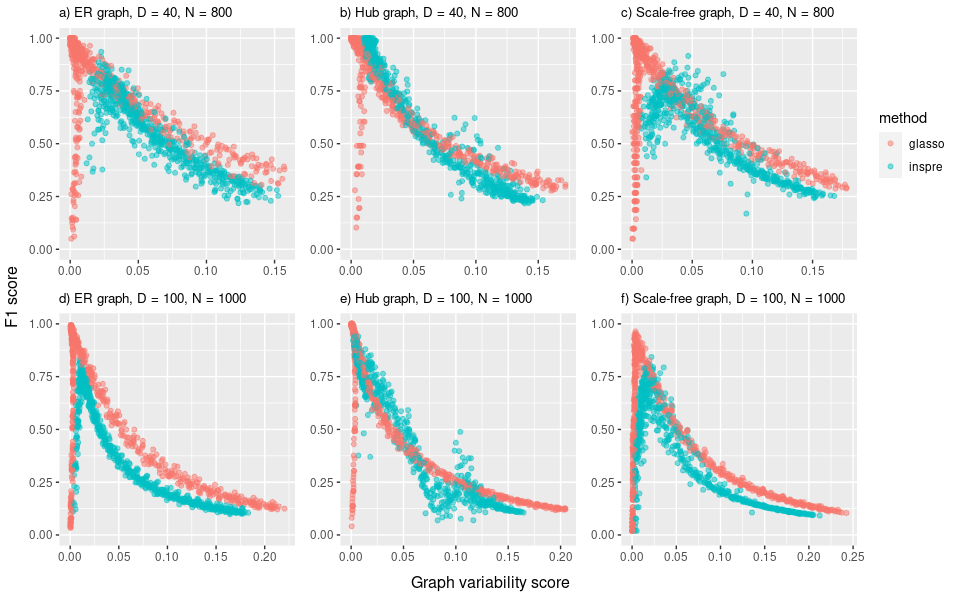
\includegraphics[width=\textwidth]{figures/figure_S1.png}
\caption{Simulations comparing inspre and glasso for various graph stuctures.}
\end{figure}

\newpage
\begin{figure}[H]\label{figureS2}
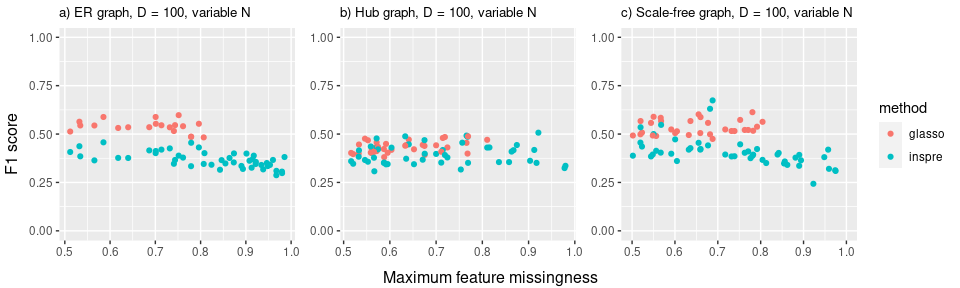
\includegraphics[width=\textwidth]{figures/figure_S2.png}
\caption{Simulations comparing inspre and glasso for various graph stuctures
with variable per-phenotype sample size.}
\end{figure}

\newpage
\begin{figure}[H]\label{figureS4}
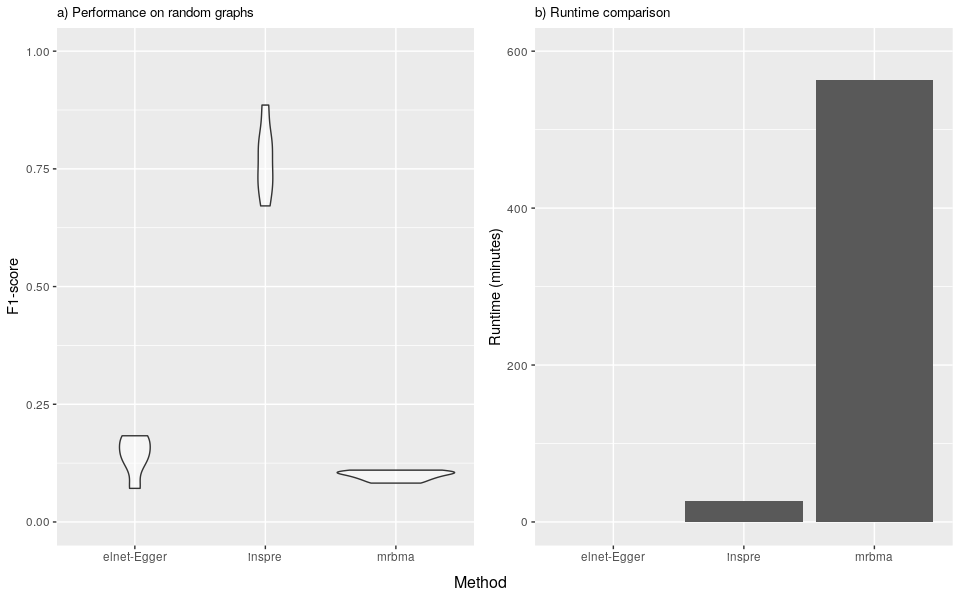
\includegraphics[width=\textwidth]{figures/figure_S4.png}
\caption{Simulations.}
\end{figure}

\newpage
\begin{figure}[H]\label{figureS3}
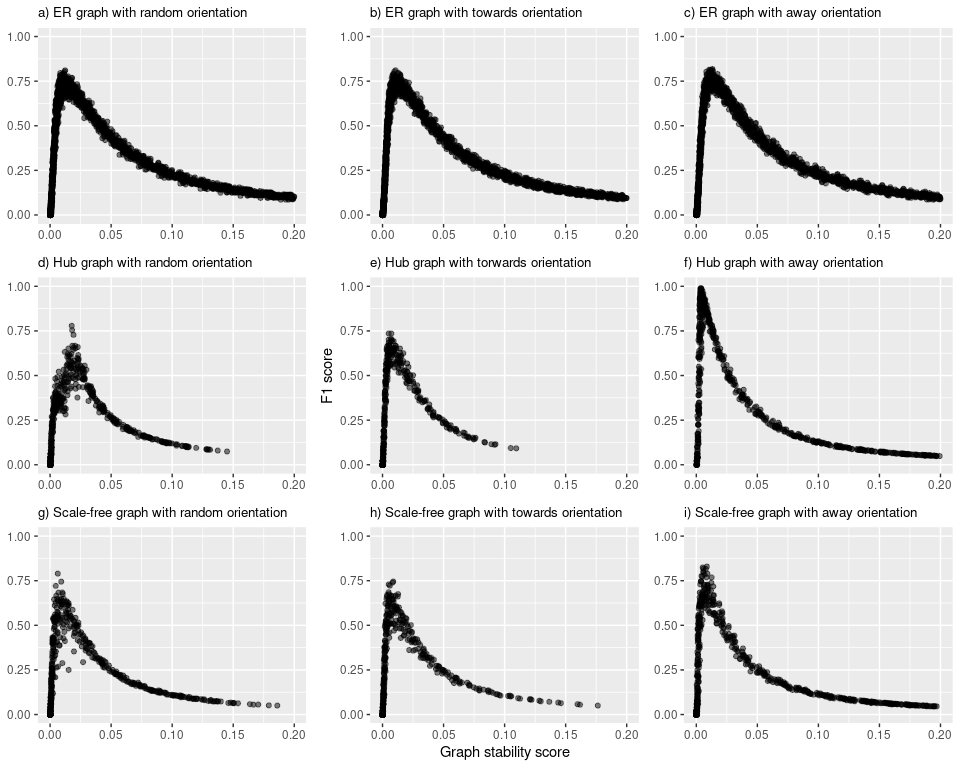
\includegraphics[width=\textwidth]{figures/figure_S3.png}
\caption{Simulations comparing inspre and glasso for various graph stuctures
with variable per-phenotype sample size.}
\end{figure}

\newpage
\begin{table}\label{table1}
\centering
\begin{tabular}{lrrrrrrrr}
\toprule
Method & stat1 & se\_stat1 & stat2 & se\_stat2 & mae1 & se\_mae1 & mae2 & se\_mae2\\
\midrule
\addlinespace[0.3em]
\multicolumn{9}{l}{\textbf{Null: Uncorrelated pleiotropy}}\\
\hspace{1em}Oracle & 0.041 & 0.006 & 0.054 & 0.007 & 0.009 & 0.000 & 0.009 & 0.000\\
\hspace{1em}W-Egger & 0.053 & 0.007 & 0.058 & 0.007 & 0.042 & 0.001 & 0.042 & 0.001\\
\hspace{1em}Egger & 0.053 & 0.007 & 0.053 & 0.007 & 0.091 & 0.002 & 0.090 & 0.002\\
\addlinespace[0.3em]
\multicolumn{9}{l}{\textbf{Null: Correlated pleiotropy}}\\
\hspace{1em}Oracle & 0.043 & 0.006 & 0.038 & 0.006 & 0.009 & 0.000 & 0.009 & 0.000\\
\hspace{1em}W-Egger & 0.051 & 0.007 & 0.068 & 0.008 & 0.044 & 0.001 & 0.047 & 0.001\\
\hspace{1em}Egger & 0.095 & 0.009 & 0.084 & 0.009 & 0.172 & 0.004 & 0.166 & 0.004\\
\addlinespace[0.3em]
\multicolumn{9}{l}{\textbf{Null: Correlated pleiotropy, unequal power}}\\
\hspace{1em}Oracle & 0.052 & 0.007 & 0.036 & 0.006 & 0.014 & 0.000 & 0.006 & 0.000\\
\hspace{1em}W-Egger & 0.087 & 0.009 & 0.029 & 0.005 & 0.053 & 0.001 & 0.080 & 0.002\\
\hspace{1em}Egger & 0.284 & 0.014 & 0.492 & 0.016 & 0.178 & 0.003 & 0.648 & 0.010\\
\bottomrule
\end{tabular}
\caption{Simulations under the two-way null.}
\end{table}

\newpage
\begin{table}\label{table2}
\centering
\begin{tabular}{lrrrrrrrr}
\toprule
Method & stat1 & se\_stat1 & stat2 & se\_stat2 & mae1 & se\_mae1 & mae2 & se\_mae2\\
\midrule
\addlinespace[0.3em]
\multicolumn{9}{l}{\textbf{Alt: Equal sample sizes, R=0.2}}\\
\hspace{1em}Oracle & 1.000 & 0.000 & 0.062 & 0.016 & 0.040 & 0.001 & 0.010 & 0.000\\
\hspace{1em}W-Egger & 0.683 & 0.030 & 0.050 & 0.014 & 0.075 & 0.003 & 0.046 & 0.002\\
\hspace{1em}Egger & 0.183 & 0.025 & 0.046 & 0.014 & 0.114 & 0.005 & 0.099 & 0.005\\
\addlinespace[0.3em]
\multicolumn{9}{l}{\textbf{Alt: Equal sample sizes, R=0.5}}\\
\hspace{1em}Oracle & 1.000 & 0.000 & 0.042 & 0.013 & 0.095 & 0.001 & 0.010 & 0.000\\
\hspace{1em}W-Egger & 0.988 & 0.007 & 0.175 & 0.025 & 0.189 & 0.004 & 0.086 & 0.004\\
\hspace{1em}Egger & 0.662 & 0.031 & 0.150 & 0.023 & 0.229 & 0.007 & 0.215 & 0.010\\
\addlinespace[0.3em]
\multicolumn{9}{l}{\textbf{Alt: Larger sample 1, R=0.2}}\\
\hspace{1em}Oracle & 1.000 & 0.000 & 0.038 & 0.012 & 0.024 & 0.001 & 0.006 & 0.000\\
\hspace{1em}W-Egger & 0.675 & 0.030 & 0.050 & 0.014 & 0.070 & 0.003 & 0.054 & 0.003\\
\hspace{1em}Egger & 0.354 & 0.031 & 0.071 & 0.017 & 0.083 & 0.004 & 0.190 & 0.013\\
\addlinespace[0.3em]
\multicolumn{9}{l}{\textbf{Alt: Larger sample 1, R=0.5}}\\
\hspace{1em}Oracle & 1.000 & 0.000 & 0.050 & 0.014 & 0.055 & 0.001 & 0.007 & 0.000\\
\hspace{1em}W-Egger & 0.992 & 0.006 & 0.075 & 0.017 & 0.148 & 0.005 & 0.086 & 0.004\\
\hspace{1em}Egger & 0.988 & 0.007 & 0.160 & 0.024 & 0.166 & 0.005 & 0.520 & 0.032\\
\addlinespace[0.3em]
\multicolumn{9}{l}{\textbf{Alt: Larger sample 2, R=0.2}}\\
\hspace{1em}Oracle & 1.000 & 0.000 & 0.058 & 0.015 & 0.065 & 0.001 & 0.015 & 0.001\\
\hspace{1em}W-Egger & 0.500 & 0.032 & 0.079 & 0.017 & 0.077 & 0.004 & 0.052 & 0.003\\
\hspace{1em}Egger & 0.079 & 0.017 & 0.092 & 0.019 & 0.237 & 0.017 & 0.068 & 0.004\\
\addlinespace[0.3em]
\multicolumn{9}{l}{\textbf{Alt: Larger sample 2, R=0.5}}\\
\hspace{1em}Oracle & 1.000 & 0.000 & 0.042 & 0.013 & 0.161 & 0.001 & 0.015 & 0.001\\
\hspace{1em}W-Egger & 0.938 & 0.016 & 0.217 & 0.027 & 0.161 & 0.006 & 0.097 & 0.004\\
\hspace{1em}Egger & 0.212 & 0.026 & 0.117 & 0.021 & 0.319 & 0.015 & 0.116 & 0.006\\
\bottomrule
\end{tabular}
\caption{Simulations under the one-way alt.}
\end{table}


\newpage
\begin{table}[H]\label{supptable1}
\centering
\begin{tabular}{lrrrrrrrr}
\toprule
p\_thresh & stat1 & se\_stat1 & stat2 & se\_stat2 & mae1 & se\_mae1 & mae2 & se\_mae2\\
\midrule
\addlinespace[0.3em]
\multicolumn{9}{l}{\textbf{Null: Uncorrelated pleiotropy}}\\
\hspace{1em}5e-04 & 0.070 & 0.008 & 0.073 & 0.008 & 0.016 & 0.000 & 0.016 & 0.000\\
\hspace{1em}5e-05 & 0.051 & 0.007 & 0.060 & 0.008 & 0.026 & 0.001 & 0.028 & 0.001\\
\hspace{1em}5e-06 & 0.053 & 0.007 & 0.058 & 0.007 & 0.042 & 0.001 & 0.042 & 0.001\\
\hspace{1em}5e-07 & 0.055 & 0.007 & 0.072 & 0.008 & 0.059 & 0.001 & 0.061 & 0.001\\
\hspace{1em}5e-08 & 0.059 & 0.007 & 0.059 & 0.007 & 0.081 & 0.002 & 0.077 & 0.002\\
\addlinespace[0.3em]
\multicolumn{9}{l}{\textbf{Null: Correlated pleiotropy}}\\
\hspace{1em}5e-04 & 0.075 & 0.008 & 0.074 & 0.008 & 0.017 & 0.000 & 0.017 & 0.000\\
\hspace{1em}5e-05 & 0.042 & 0.006 & 0.051 & 0.007 & 0.027 & 0.001 & 0.027 & 0.001\\
\hspace{1em}5e-06 & 0.051 & 0.007 & 0.068 & 0.008 & 0.044 & 0.001 & 0.047 & 0.001\\
\hspace{1em}5e-07 & 0.041 & 0.006 & 0.064 & 0.008 & 0.065 & 0.002 & 0.066 & 0.002\\
\hspace{1em}5e-08 & 0.039 & 0.006 & 0.058 & 0.007 & 0.088 & 0.002 & 0.088 & 0.002\\
\addlinespace[0.3em]
\multicolumn{9}{l}{\textbf{Null: Correlated pleiotropy, unequal power}}\\
\hspace{1em}5e-04 & 0.078 & 0.008 & 0.366 & 0.015 & 0.039 & 0.001 & 0.033 & 0.001\\
\hspace{1em}5e-05 & 0.086 & 0.009 & 0.144 & 0.011 & 0.045 & 0.001 & 0.050 & 0.001\\
\hspace{1em}5e-06 & 0.087 & 0.009 & 0.029 & 0.005 & 0.053 & 0.001 & 0.080 & 0.002\\
\hspace{1em}5e-07 & 0.073 & 0.008 & 0.049 & 0.007 & 0.060 & 0.001 & 0.187 & 0.006\\
\hspace{1em}5e-08 & 0.067 & 0.008 & 0.075 & 0.008 & 0.067 & 0.002 & 0.373 & 0.013\\
\bottomrule
\end{tabular}
\caption{Simulations under the two-way null for various p-value thresholds.}
\end{table}

\begin{table}[H]\label{supptable2}
\centering
\begin{tabular}{lrrrrrrrr}
\toprule
p\_thresh & stat1 & se\_stat1 & stat2 & se\_stat2 & mae1 & se\_mae1 & mae2 & se\_mae2\\
\midrule
\addlinespace[0.3em]
\multicolumn{9}{l}{\textbf{Alt: Equal sample sizes, R=0.2}}\\
\hspace{1em}5e-04 & 1.000 & 0.000 & 0.150 & 0.023 & 0.023 & 0.001 & 0.020 & 0.001\\
\hspace{1em}5e-05 & 0.988 & 0.007 & 0.079 & 0.017 & 0.048 & 0.002 & 0.031 & 0.001\\
\hspace{1em}5e-06 & 0.683 & 0.030 & 0.050 & 0.014 & 0.075 & 0.003 & 0.046 & 0.002\\
\hspace{1em}5e-07 & 0.375 & 0.031 & 0.042 & 0.013 & 0.089 & 0.004 & 0.064 & 0.003\\
\hspace{1em}5e-08 & 0.246 & 0.028 & 0.033 & 0.012 & 0.102 & 0.005 & 0.083 & 0.004\\
\addlinespace[0.3em]
\multicolumn{9}{l}{\textbf{Alt: Equal sample sizes, R=0.5}}\\
\hspace{1em}5e-04 & 1.000 & 0.000 & 0.596 & 0.032 & 0.058 & 0.002 & 0.051 & 0.002\\
\hspace{1em}5e-05 & 1.000 & 0.000 & 0.288 & 0.029 & 0.108 & 0.003 & 0.065 & 0.002\\
\hspace{1em}5e-06 & 0.988 & 0.007 & 0.175 & 0.025 & 0.189 & 0.004 & 0.086 & 0.004\\
\hspace{1em}5e-07 & 0.850 & 0.023 & 0.142 & 0.023 & 0.229 & 0.006 & 0.120 & 0.006\\
\hspace{1em}5e-08 & 0.612 & 0.032 & 0.079 & 0.017 & 0.239 & 0.008 & 0.155 & 0.007\\
\addlinespace[0.3em]
\multicolumn{9}{l}{\textbf{Alt: Larger sample 1, R=0.2}}\\
\hspace{1em}5e-04 & 0.929 & 0.017 & 0.133 & 0.022 & 0.050 & 0.002 & 0.018 & 0.001\\
\hspace{1em}5e-05 & 0.812 & 0.025 & 0.058 & 0.015 & 0.060 & 0.003 & 0.028 & 0.001\\
\hspace{1em}5e-06 & 0.675 & 0.030 & 0.050 & 0.014 & 0.070 & 0.003 & 0.054 & 0.003\\
\hspace{1em}5e-07 & 0.467 & 0.032 & 0.046 & 0.014 & 0.078 & 0.004 & 0.107 & 0.006\\
\hspace{1em}5e-08 & 0.358 & 0.031 & 0.062 & 0.016 & 0.087 & 0.004 & 0.161 & 0.010\\
\addlinespace[0.3em]
\multicolumn{9}{l}{\textbf{Alt: Larger sample 1, R=0.5}}\\
\hspace{1em}5e-04 & 1.000 & 0.000 & 0.433 & 0.032 & 0.095 & 0.003 & 0.037 & 0.001\\
\hspace{1em}5e-05 & 1.000 & 0.000 & 0.242 & 0.028 & 0.118 & 0.004 & 0.055 & 0.002\\
\hspace{1em}5e-06 & 0.992 & 0.006 & 0.075 & 0.017 & 0.148 & 0.005 & 0.086 & 0.004\\
\hspace{1em}5e-07 & 0.958 & 0.013 & 0.085 & 0.018 & 0.157 & 0.005 & 0.185 & 0.010\\
\hspace{1em}5e-08 & 0.896 & 0.020 & 0.104 & 0.020 & 0.165 & 0.006 & 0.334 & 0.018\\
\addlinespace[0.3em]
\multicolumn{9}{l}{\textbf{Alt: Larger sample 2, R=0.2}}\\
\hspace{1em}5e-04 & 1.000 & 0.000 & 0.092 & 0.019 & 0.039 & 0.001 & 0.041 & 0.002\\
\hspace{1em}5e-05 & 1.000 & 0.000 & 0.088 & 0.018 & 0.043 & 0.002 & 0.045 & 0.002\\
\hspace{1em}5e-06 & 0.500 & 0.032 & 0.079 & 0.017 & 0.077 & 0.004 & 0.052 & 0.003\\
\hspace{1em}5e-07 & 0.162 & 0.024 & 0.096 & 0.019 & 0.135 & 0.006 & 0.058 & 0.003\\
\hspace{1em}5e-08 & 0.080 & 0.018 & 0.088 & 0.018 & 0.216 & 0.012 & 0.066 & 0.003\\
\addlinespace[0.3em]
\multicolumn{9}{l}{\textbf{Alt: Larger sample 2, R=0.5}}\\
\hspace{1em}5e-04 & 1.000 & 0.000 & 0.246 & 0.028 & 0.146 & 0.002 & 0.072 & 0.003\\
\hspace{1em}5e-05 & 1.000 & 0.000 & 0.212 & 0.026 & 0.098 & 0.003 & 0.078 & 0.003\\
\hspace{1em}5e-06 & 0.938 & 0.016 & 0.217 & 0.027 & 0.161 & 0.006 & 0.097 & 0.004\\
\hspace{1em}5e-07 & 0.435 & 0.032 & 0.183 & 0.025 & 0.259 & 0.011 & 0.106 & 0.005\\
\hspace{1em}5e-08 & 0.150 & 0.023 & 0.146 & 0.023 & 0.343 & 0.016 & 0.118 & 0.006\\
\bottomrule
\end{tabular}
\caption{Simulations under the one-way alt for various p-value thresholds.}
\end{table}

\end{document}